\documentclass{article}

\usepackage{fullpage}
\usepackage{amsmath,amsfonts,amsthm,amssymb}
\usepackage{graphicx}
\usepackage{color}
\usepackage{listings}
\usepackage{color}

\usepackage{amsmath}
\usepackage{algorithm}
\usepackage[noend]{algpseudocode}

\makeatletter
\def\BState{\State\hskip-\ALG@thistlm}
\makeatother


\definecolor{dkgreen}{rgb}{0,0.6,0}
\definecolor{gray}{rgb}{0.5,0.5,0.5}
\definecolor{mauve}{rgb}{0.58,0,0.82}

\lstset{frame=tb,
  language=Java,
  aboveskip=3mm,
  belowskip=3mm,
  showstringspaces=false,
  columns=flexible,
  basicstyle={\small\ttfamily},
  numbers=none,
  numberstyle=\tiny\color{gray},
  keywordstyle=\color{blue},
  commentstyle=\color{dkgreen},
  stringstyle=\color{mauve},
  breaklines=true,
  breakatwhitespace=true,
  tabsize=3
}

\begin{document}
\title{CS 457, Data Structures and Algorithms I\\
Fourth Problem Set}
\date{November 22, 2016}
\maketitle
\begin{center}
\textbf{Due on December 2. Collaboration is not allowed. Contact me directly with any questions.}
\end{center}
\begin{enumerate}

\item (10 pts) Given the pattern $P=abbababbaaab$ and the text string $T=aaababaabaababaababbababbaaabbabab$
\begin{itemize}
\item[a)] Construct the string matching automaton for $P$, and illustrate its operation on $T$.

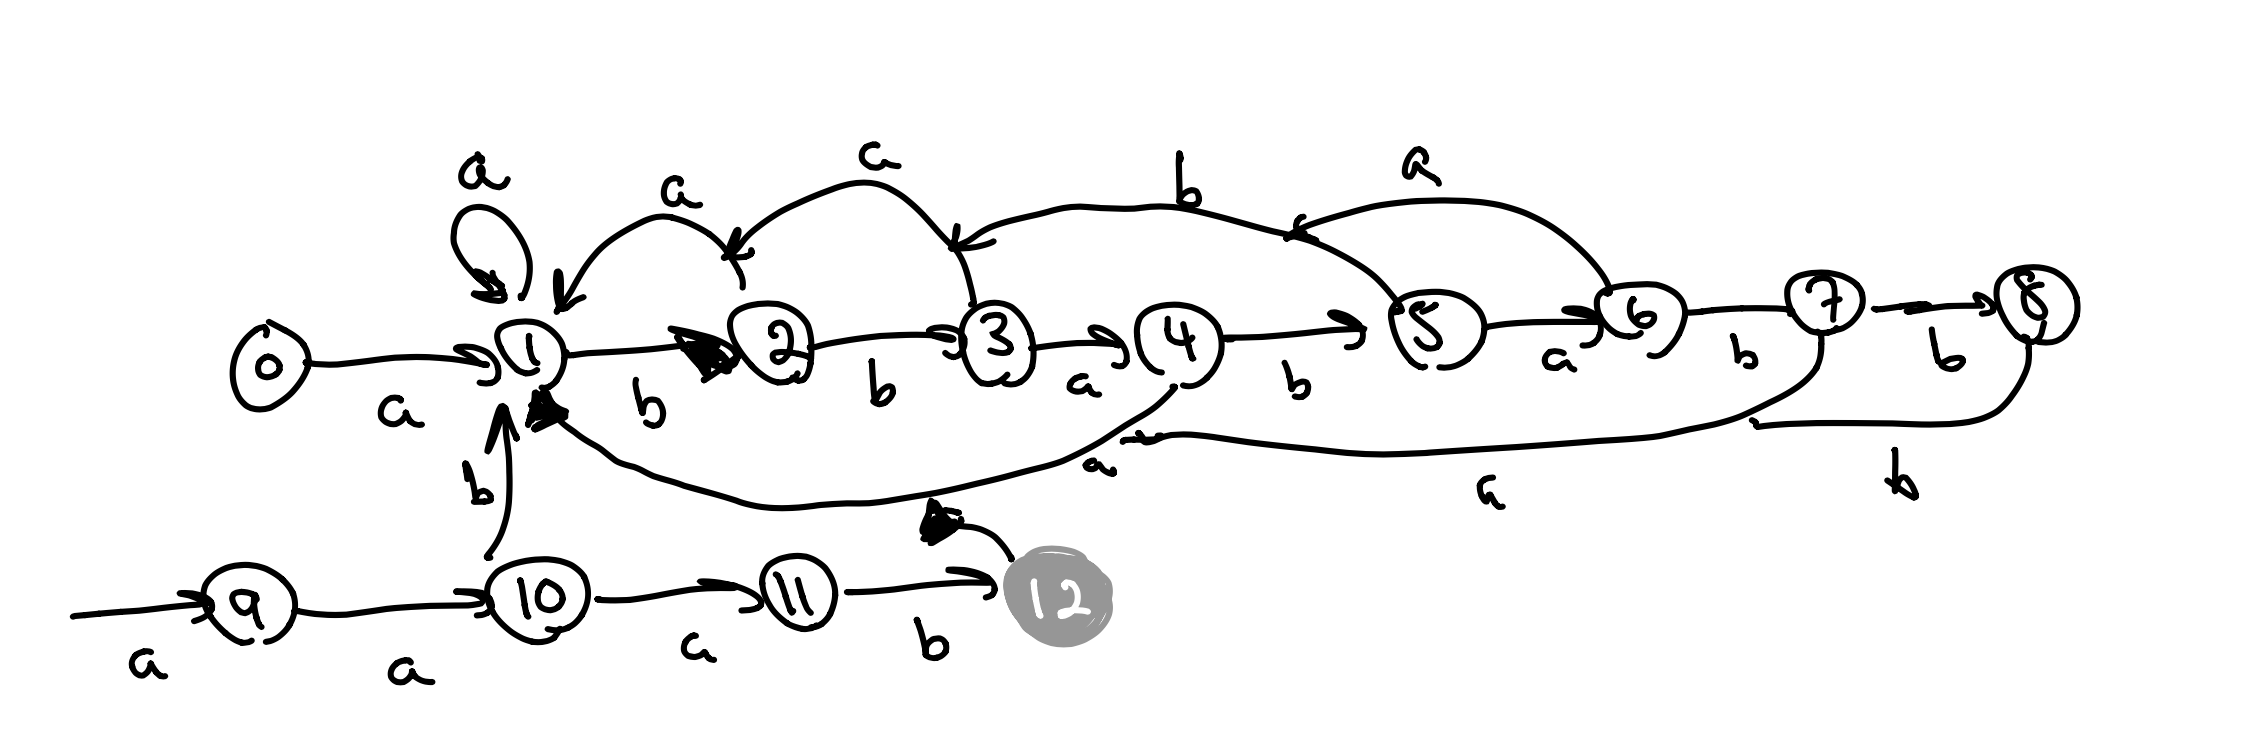
\includegraphics[scale=0.4]{automata}

The state-transition diagram above accepts all strings with $abbababbaaab$ and finds the match. Running through $T=aaababaabaababaababbababbaaabbabab$, we can see that it loops for the first 3 characters $a$ in state $1$. Afterwards, it takes in $b$ and goes to state $2$, but goes back to state $1$ since the next character is $a$. It keeps going back to state $1$ constantly until it reaches the 19th character 
$T=aaababaabaababaab\textcolor{red}{abbababbaaab}babab$ starting with $a$. The automata then smoothly goes from the starting state at 1 to 12. 
\newpage

\item[b)] Compute the prefix function $\pi$ for $P$, and illustrate the operation of the KMP algorithm on $T$.

\begin{center}
\begin{tabular}{ c c c c c c c c c c c c c}
 i & 1 & 2 & 3 & 4 & 5 & 6 & 7 & 8 & 9 & 10 & 11 & 12 \\ 
 P[i] & a & b & b & a & b & a & b & b & a & a & a & b \\
 $\pi$ & 0&0&0&1&2&1&0&3&4&1&1&2
\end{tabular}
\end{center}

\end{itemize}

Given $T=aaababaabaababaababbababbaaabbabab$

It will compare $T=\textcolor{red}{aa}ababaabaababaababbababbaaabbabab$

The algorithm then checks if the prefix and suffix are the same. Since they aren't a match, it will continue to do so until it reaches a comparison where it doesn't match and the prefix function is greater than 0. It will use the non-matching string as a pivot point where the character after the prefix is compared. If they are valid, it continues to do so until it either reaches a non match, in which it starts its comparison over again from that point or finds the match seen below.

$T=aaababaabaababaab\textcolor{red}{abbababbaaab}babab$

(There aren't 2 $b$'s until it actually reaches the string, thus the string matching isn't used until then, which in this case it reaches the match)
\newpage


\item (15 pts) Write an algorithm that reads characters one at a time and reports at each instant if the current string is a palindrome. Hint: Use the Rabin-Karp hashing idea.

\begin{algorithm}
\caption{Computes if current string is a palindrome at each substring}\label{euclid}
\begin{algorithmic}[1]
\Procedure{COMPUTE-PALINDROME(P)}{}
\BState $\textit{m} \gets \text{P.length}$
\BState let $\pi$[1\dotso m] be a new array
\BState $\pi$[1] = $true$ //false by default
\BState k = 0
\BState \textbf{for}  $q$ = 2 \textbf{to} $m$
\State \textbf{while} $k > 0$ and $P[k+1] \neq P[q]$
\State \hspace{9mm} $k = \pi[k]$
\State \textbf{if} $P[k+1] == P[q]$
\State \hspace{9mm} $k = k + 1$
\State \textbf{if}  $ k == q/2 $
\State \hspace{9mm} $\pi[q] = true$
\BState \textbf{return} $\pi$
\EndProcedure
\end{algorithmic}
\end{algorithm}


\newpage

\item (15 pts) A directed Eulerian cycle is a directed cycle that contains each edge exactly once. Write an algorithm that finds a directed Eulerian cycle or reports that no such cycle exists. Hint: Prove that a strongly-connected digraph $G$ has a directed Eulerian cycle if and only if each vertex has its indegree equal to its outdegree.
\begin{lstlisting}
isDirectedEurleianCycle(G): 

if(G has no edges) {
  return false
}

for all vertices in G
  if(outdegree(v) != indegree(v)) {
    return false;
  }
  
int cycles = DFS() where DFS returns number of cycles 

if(cycles == G.getNumberofEdges()) {
  return true;
}
\end{lstlisting}
\newpage

\item (15 pts) Given a DAG and two vertices $v$ and $w$, find a shortest ancestral path between $v$ and $w$. An ancestral path between $v$ and $w$ is a common ancestor $x$ along with a shortest directed path from $v$ to $x$ and a shortest directed path from $w$ to $x$. A shortest ancestral path in the ancestral path whose total length is minimized. Warmup: Find a DAG where the shortest ancestral path goes to a common ancestor $x$ that is not LCA. 

\begin{lstlisting}
ShortestAncestralPath(v, w):
//traverse to root
while(notRoot) {
	visited[v] = true;
	v = parent[v];
}

//traverse path back to root and checks if state is visited
shortestPath = null;
while(shortestPath != root) {
	if(visited[w]) {
		shortestPath = w
	}
	w = parent[w]
}
return shortestPath
\end{lstlisting}



\newpage

\item (15 pts) A bridge in a graph is an edges that, if removed, would increase the number of connected components. A graph that has no bridges is said to be {\em two-edge connected}. Write a linear time DFS-based algorithm for finding all bridges in a graph or determining whether it is not two-edge connected.

\begin{lstlisting}
count = 0;

initBridge() : 
  for all x in temp
    temp[x] = false;
    
FINDINGBRIDGES(u, v):
  temp[v] = true;
  y[v] = temp[v];
  for x in G adjacent to u:
    if(temp[x]) 
      FINDBRIDGES(v, x);
      y[v] = min(y[v], y[w]);
      if(x[v] == x[w]) 
        print(v "-" w "is a bridge")
      else if(x != u) 
      y[v] = min(y[v], temp[x]);
\end{lstlisting}

\newpage

\item (15 pts) Given a connected edge-weighted graph $G$ and a specified set of edges $S$ that contains no cycles, provide an algorithm that finds a minimum-weight spanning tree among all the spanning trees that contain all the edges in $S$. Also, provide an upper bound on the running time of your algorithm, and prove its correctness.

\begin{lstlisting}
KRUSKALMODIFIED(G) :
x = null;
for all v in G.V:
    CREATE-SET(v)
for all (u, v) in S ordered by weight(u, v), increasing:
    if(set(u) != set(v))
      x = x U {(u, v)}
      union(u, v)
\end{lstlisting}
The algorithm itself should run in $O(S log V)$ time, where S is the set of edges. For the initial part of the algorithm, $x = null$ will take constant time. The $CREATE-SET(v)$ will take $O(SlogS)$ time as it creates a set. (Hand wavy - refine). At each iteration in the second for loop, it checks whether $u$ and $v$ are not in the same set, which takes $O(N)$. Thus the toal running time of the algorithm is then $O(SlogV)$ as the upper bound. 

\newpage

\item (15 pts) Design an algorithm that, given two strings, determines whether one is a cyclic rotation of the other (e.g., ``example'' and ``leexamp'').

\begin{lstlisting}
public boolean isCyclicRotation(String s1, String s2) {
	if(s1.length != s2.length) {
		return false;
	}
	String concatStr1 = s1 + s1;
	String concatStr2 = s2 + s2;
	if(!(concatStr1.contains(s2) || concatStr2.contains(s1) ){
		return false;
	}
	return true;
}
\end{lstlisting}

\end{enumerate}
\end{document}